\documentclass{standalone}
\usepackage{tikz}
\usetikzlibrary{patterns, positioning}


\begin{document}
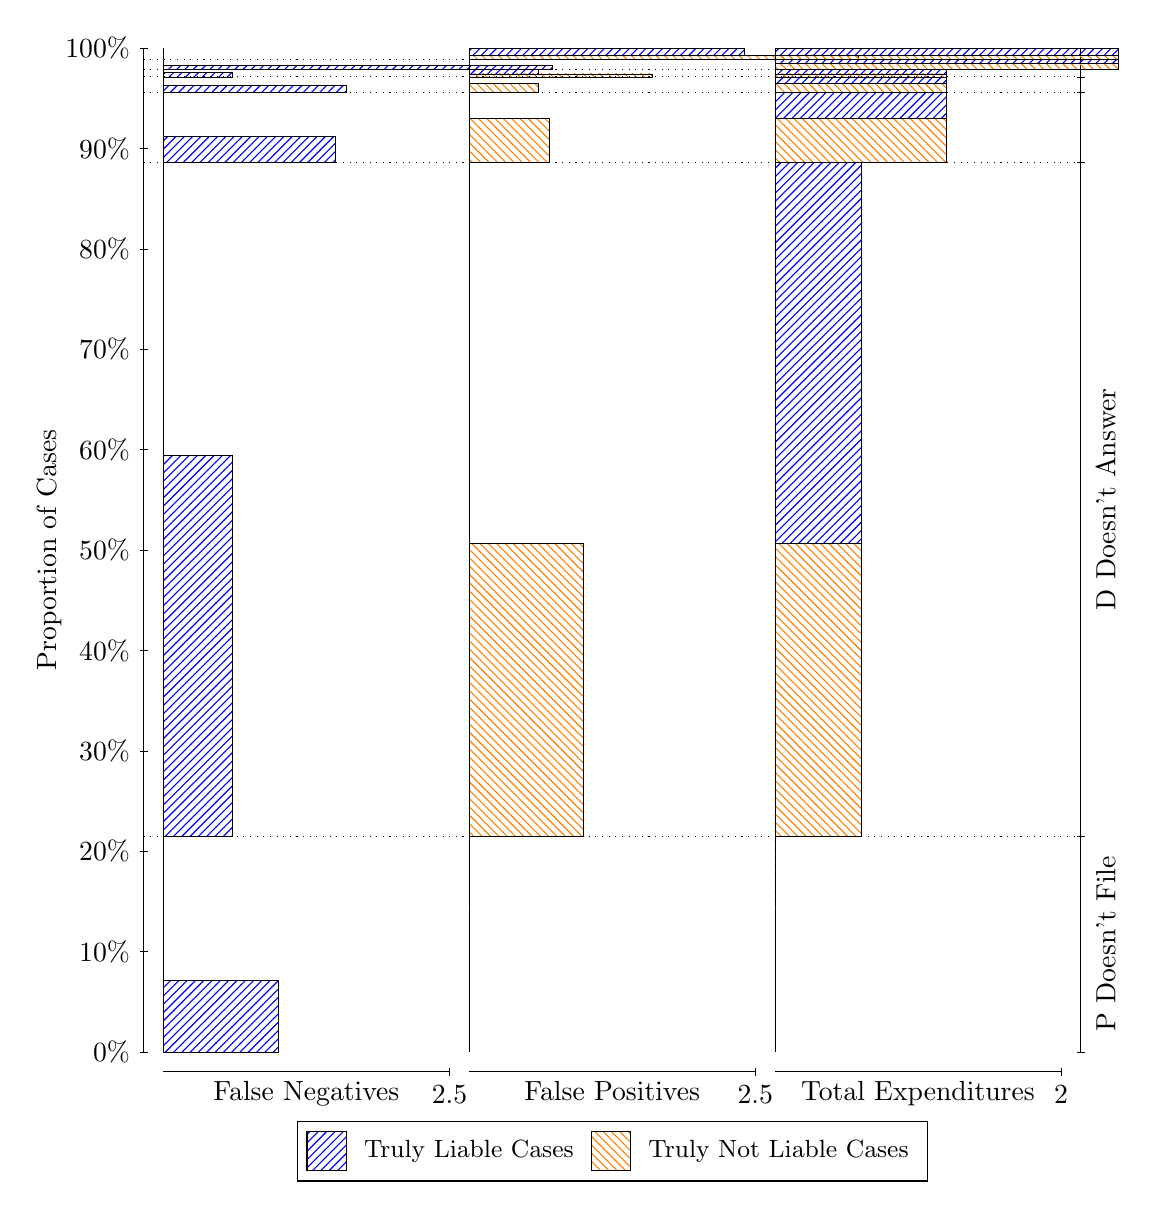
\begin{tikzpicture}
\draw[black, very thin] (1.5,1.75) -- (1.5,14.5);
\node[rotate=90, text=black, anchor=center] at (0.3, 8.125) {Proportion of Cases};
\draw[black, very thin] (1.45,1.75) -- (1.55,1.75);
\node[text=black, anchor=east] at (1.45, 1.75) {0\%};
\draw[black, very thin] (1.45,3.025) -- (1.55,3.025);
\node[text=black, anchor=east] at (1.45, 3.025) {10\%};
\draw[black, very thin] (1.45,4.3) -- (1.55,4.3);
\node[text=black, anchor=east] at (1.45, 4.3) {20\%};
\draw[black, very thin] (1.45,5.575) -- (1.55,5.575);
\node[text=black, anchor=east] at (1.45, 5.575) {30\%};
\draw[black, very thin] (1.45,6.85) -- (1.55,6.85);
\node[text=black, anchor=east] at (1.45, 6.85) {40\%};
\draw[black, very thin] (1.45,8.125) -- (1.55,8.125);
\node[text=black, anchor=east] at (1.45, 8.125) {50\%};
\draw[black, very thin] (1.45,9.4) -- (1.55,9.4);
\node[text=black, anchor=east] at (1.45, 9.4) {60\%};
\draw[black, very thin] (1.45,10.675) -- (1.55,10.675);
\node[text=black, anchor=east] at (1.45, 10.675) {70\%};
\draw[black, very thin] (1.45,11.95) -- (1.55,11.95);
\node[text=black, anchor=east] at (1.45, 11.95) {80\%};
\draw[black, very thin] (1.45,13.225) -- (1.55,13.225);
\node[text=black, anchor=east] at (1.45, 13.225) {90\%};
\draw[black, very thin] (1.45,14.5) -- (1.55,14.5);
\node[text=black, anchor=east] at (1.45, 14.5) {100\%};

\draw[black, very thin] (13.4,1.75) -- (13.4,14.5);
\draw[black, very thin] (13.35,1.75) -- (13.45,1.75);
\node[anchor=west] at (13.35, 1.75) {};
\draw[black, very thin] (13.35,4.492) -- (13.45,4.492);
\node[anchor=west] at (13.35, 4.492) {};
\draw[black, very thin] (13.35,13.044) -- (13.45,13.044);
\node[anchor=west] at (13.35, 13.044) {};
\draw[black, very thin] (13.35,13.939) -- (13.45,13.939);
\node[anchor=west] at (13.35, 13.939) {};
\draw[black, very thin] (13.35,14.133) -- (13.45,14.133);
\node[anchor=west] at (13.35, 14.133) {};
\draw[black, very thin] (13.35,14.227) -- (13.45,14.227);
\node[anchor=west] at (13.35, 14.227) {};
\draw[black, very thin] (13.35,14.356) -- (13.45,14.356);
\node[anchor=west] at (13.35, 14.356) {};
\draw[black, very thin] (13.35,14.5) -- (13.45,14.5);
\node[anchor=west] at (13.35, 14.5) {};

\draw[black, very thin, pattern color=blue, pattern=north east lines] (1.75,1.75) rectangle (3.2033,2.6583);
\draw[black, very thin, pattern color=orange, pattern=north west lines] (1.75,2.6583) rectangle (1.75,4.492);
\draw[black, very thin, pattern color=blue, pattern=north east lines] (1.75,4.492) rectangle (2.622,9.3298);
\draw[black, very thin, pattern color=orange, pattern=north west lines] (1.75,9.3298) rectangle (1.75,13.044);
\draw[black, very thin, pattern color=blue, pattern=north east lines] (1.75,13.044) rectangle (3.93,13.379);
\draw[black, very thin, pattern color=orange, pattern=north west lines] (1.75,13.379) rectangle (1.75,13.939);
\draw[black, very thin, pattern color=blue, pattern=north east lines] (1.75,13.939) rectangle (4.0753,14.026);
\draw[black, very thin, pattern color=orange, pattern=north west lines] (1.75,14.026) rectangle (1.75,14.133);
\draw[black, very thin, pattern color=blue, pattern=north east lines] (1.75,14.133) rectangle (2.622,14.189);
\draw[black, very thin, pattern color=orange, pattern=north west lines] (1.75,14.189) rectangle (1.75,14.227);
\draw[black, very thin, pattern color=blue, pattern=north east lines] (1.75,14.227) rectangle (6.6913,14.282);
\draw[black, very thin, pattern color=orange, pattern=north west lines] (1.75,14.282) rectangle (1.75,14.356);
\draw[black, very thin, pattern color=orange, pattern=north west lines] (1.75,14.356) rectangle (1.75,14.403);
\draw[black, very thin, pattern color=blue, pattern=north east lines] (1.75,14.403) rectangle (1.75,14.5);
\draw[black, very thin, pattern color=orange, pattern=north west lines] (5.6333,1.75) rectangle (5.6333,3.5837);
\draw[black, very thin, pattern color=blue, pattern=north east lines] (5.6333,3.5837) rectangle (5.6333,4.492);
\draw[black, very thin, pattern color=orange, pattern=north west lines] (5.6333,4.492) rectangle (7.0867,8.2062);
\draw[black, very thin, pattern color=blue, pattern=north east lines] (5.6333,8.2062) rectangle (5.6333,13.044);
\draw[black, very thin, pattern color=orange, pattern=north west lines] (5.6333,13.044) rectangle (6.6507,13.604);
\draw[black, very thin, pattern color=blue, pattern=north east lines] (5.6333,13.604) rectangle (5.6333,13.939);
\draw[black, very thin, pattern color=orange, pattern=north west lines] (5.6333,13.939) rectangle (6.5053,14.047);
\draw[black, very thin, pattern color=blue, pattern=north east lines] (5.6333,14.047) rectangle (5.6333,14.133);
\draw[black, very thin, pattern color=orange, pattern=north west lines] (5.6333,14.133) rectangle (7.9587,14.172);
\draw[black, very thin, pattern color=blue, pattern=north east lines] (5.6333,14.172) rectangle (6.5053,14.227);
\draw[black, very thin, pattern color=orange, pattern=north west lines] (5.6333,14.227) rectangle (5.6333,14.301);
\draw[black, very thin, pattern color=blue, pattern=north east lines] (5.6333,14.301) rectangle (5.6333,14.356);
\draw[black, very thin, pattern color=orange, pattern=north west lines] (5.6333,14.356) rectangle (10.575,14.403);
\draw[black, very thin, pattern color=blue, pattern=north east lines] (5.6333,14.403) rectangle (9.1213,14.5);
\draw[black, very thin, pattern color=orange, pattern=north west lines] (9.5167,1.75) rectangle (9.5167,3.5837);
\draw[black, very thin, pattern color=blue, pattern=north east lines] (9.5167,3.5837) rectangle (9.5167,4.492);
\draw[black, very thin, pattern color=orange, pattern=north west lines] (9.5167,4.492) rectangle (10.607,8.2062);
\draw[black, very thin, pattern color=blue, pattern=north east lines] (9.5167,8.2062) rectangle (10.607,13.044);
\draw[black, very thin, pattern color=orange, pattern=north west lines] (9.5167,13.044) rectangle (11.697,13.604);
\draw[black, very thin, pattern color=blue, pattern=north east lines] (9.5167,13.604) rectangle (11.697,13.939);
\draw[black, very thin, pattern color=orange, pattern=north west lines] (9.5167,13.939) rectangle (11.697,14.047);
\draw[black, very thin, pattern color=blue, pattern=north east lines] (9.5167,14.047) rectangle (11.697,14.133);
\draw[black, very thin, pattern color=orange, pattern=north west lines] (9.5167,14.133) rectangle (11.697,14.172);
\draw[black, very thin, pattern color=blue, pattern=north east lines] (9.5167,14.172) rectangle (11.697,14.227);
\draw[black, very thin, pattern color=orange, pattern=north west lines] (9.5167,14.227) rectangle (13.877,14.301);
\draw[black, very thin, pattern color=blue, pattern=north east lines] (9.5167,14.301) rectangle (13.877,14.356);
\draw[black, very thin, pattern color=orange, pattern=north west lines] (9.5167,14.356) rectangle (13.877,14.403);
\draw[black, very thin, pattern color=blue, pattern=north east lines] (9.5167,14.403) rectangle (13.877,14.5);
\draw[black, dotted] (1.5,4.492) -- (13.4,4.492);
\draw[black, dotted] (1.5,13.044) -- (13.4,13.044);
\draw[black, dotted] (1.5,13.939) -- (13.4,13.939);
\draw[black, dotted] (1.5,14.133) -- (13.4,14.133);
\draw[black, dotted] (1.5,14.227) -- (13.4,14.227);
\draw[black, dotted] (1.5,14.356) -- (13.4,14.356);
\draw[black, very thin] (1.75,1.5) -- (5.3833,1.5);
\node[text=black, anchor=north] at (3.5667, 1.5) {False Negatives};
\draw[black, very thin] (5.3833,1.45) -- (5.3833,1.55);
\node[text=black, anchor=north] at (5.3833, 1.45) {2.5};

\draw[black, very thin] (5.6333,1.5) -- (9.2667,1.5);
\node[text=black, anchor=north] at (7.45, 1.5) {False Positives};
\draw[black, very thin] (9.2667,1.45) -- (9.2667,1.55);
\node[text=black, anchor=north] at (9.2667, 1.45) {2.5};

\draw[black, very thin] (9.5167,1.5) -- (13.15,1.5);
\node[text=black, anchor=north] at (11.333, 1.5) {Total Expenditures};
\draw[black, very thin] (13.15,1.45) -- (13.15,1.55);
\node[text=black, anchor=north] at (13.15, 1.45) {2};

\node[text=black, centered, rotate=90] at (13.72, 3.121) {P Doesn't File};
\node[text=black, centered, rotate=90] at (13.72, 8.768) {D Doesn't Answer};






\draw (7.449999999999999,1.5) node[draw=none] (baseCoordinate) {};
\begin{scope}[align=center]
        \matrix[scale=0.5, draw=black, below=0.5cm of baseCoordinate, nodes={draw}, column sep=0.1cm]{
            \node[rectangle, draw, minimum width=0.5cm, minimum height=0.5cm, pattern color=blue, pattern=north east lines] {}; &
            \node[draw=none, font=\small, text=black] (B) {Truly Liable Cases}; &
            \node[rectangle, draw, minimum width=0.5cm, minimum height=0.5cm, pattern color=orange, pattern=north west lines] {}; &
            \node[draw=none, font=\small, text=black] (B) {Truly Not Liable Cases}; \\
            };
\end{scope}

\end{tikzpicture}
\end{document}